\section{Crew interfaces}
\label{sec:interfaces}

\begin{figure*}[t]
  \centering
  \begin{subfigure}[b]{0.615\textwidth}\centering
    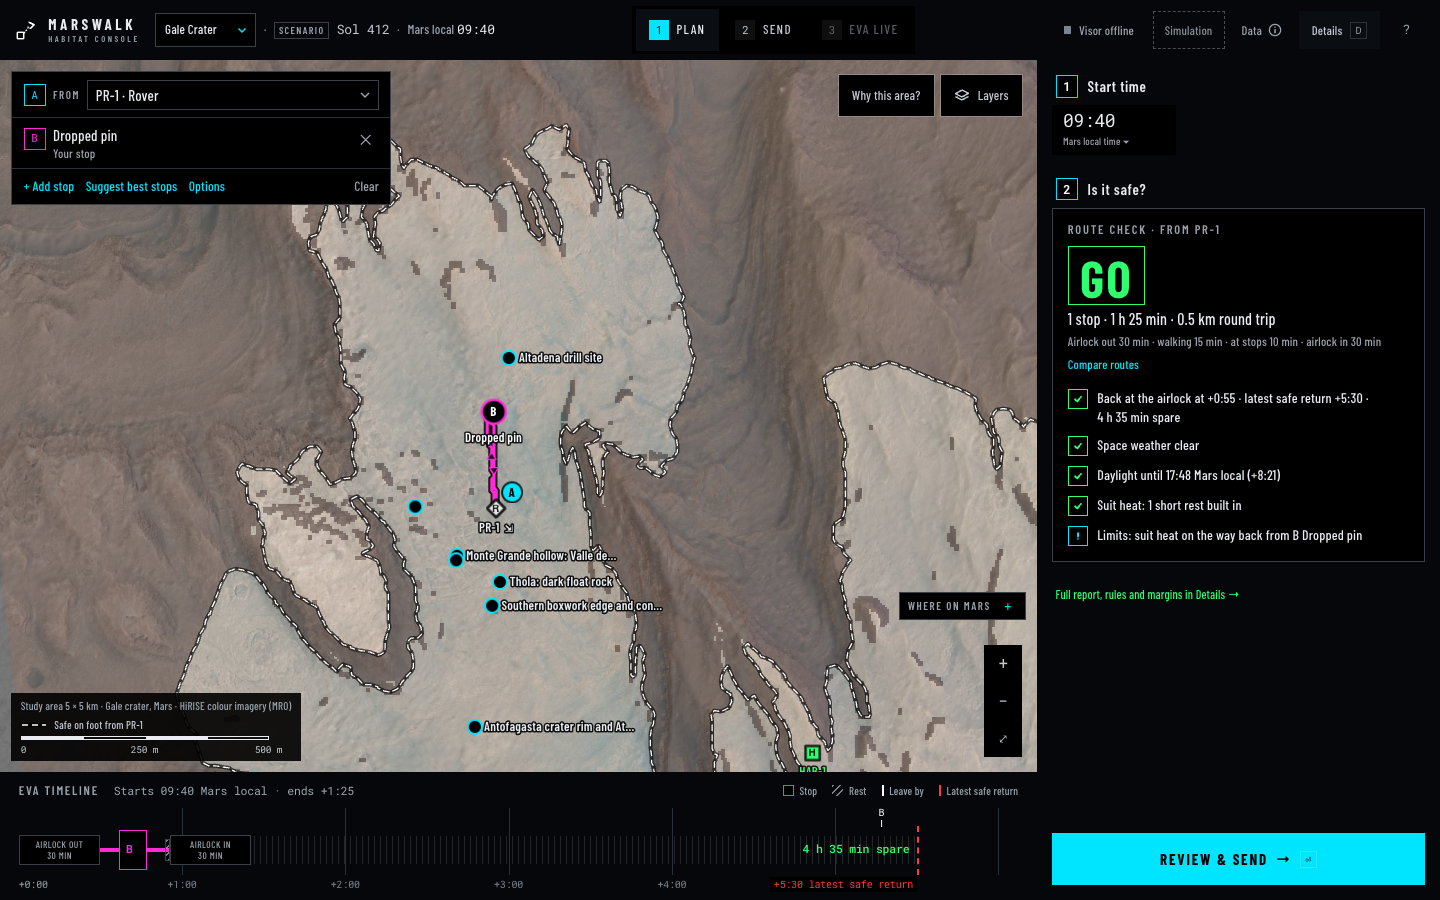
\includegraphics[width=\textwidth]{console-go.png}
    \caption{Plan mode: a \go verdict for a pin staged from PR-1.}
  \end{subfigure}\hfill
  \begin{subfigure}[b]{0.365\textwidth}\centering
    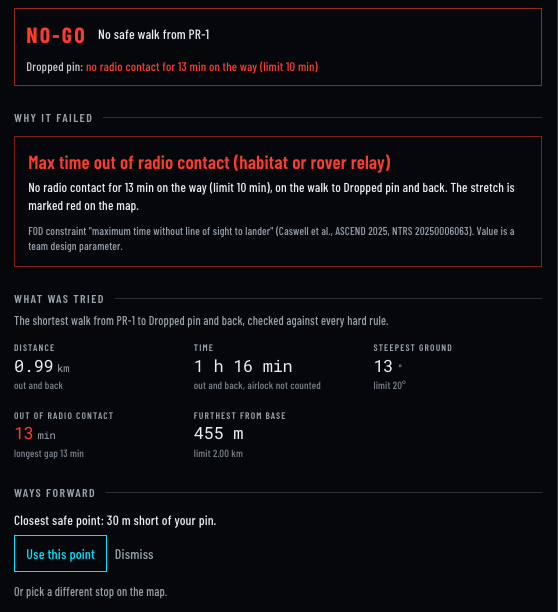
\includegraphics[width=\textwidth]{console-nogo-details.png}
    \caption{A \nogo explained.}
  \end{subfigure}
  \caption{Habitat console at Gale. (a) The IV picks a base and drops a pin. The verdict card lists the latest safe return, space weather, daylight and suit-heat rests. The dashed outline is the area walkable under the per-cell constraints, the magenta line is the route, and the timeline shows the airlock periods and the latest safe return. (b) For a pin in a radio shadow, the details drawer names the failing rule (13\,min without contact against a limit of 10) and its source, reports what was tried, and offers the closest safe point, which the engine has re-planned and confirmed.}
  \label{fig:console}
\end{figure*}

\paragraph{Habitat console.} The console asks one question at a time and moves through three modes: \emph{Plan}, \emph{Send} and \emph{EVA live} (\cref{fig:console}). Interaction follows familiar consumer map conventions. The IV sets a base and destinations, searches named places or drops a pin anywhere, and each pin gets an immediate safety preview. Science stations appear as suggested places, but any destination the IV picks is treated as must-visit: if it is infeasible, the console explains why instead of dropping it. The verdict comes first, in plain terms such as ``what limits this walk'', ``leave-by time'' and ``no safe walk from here''. A ``Why this area?'' sequence shrinks the walkable area one constraint at a time and cites the source of each limit. For a \nogo, the console marks the failing stretch of the route in red and offers two ways forward: the closest safe point and a better rover position. A rules view lists all twelve constraints with their evidence classes, and an evidence panel states what is measured and what is assumed. In the end-to-end test the verdict appears 2.1\,s after page load with no clicks, a plan reaches crew acceptance in three clicks, and an emergency re-route takes two.

\newcommand{\phoneshot}[2]{\tikz[baseline]{\node[inner sep=0pt] (img) {\includegraphics[height=#2]{#1}};
  \draw[ink, line width=2.2pt, rounded corners=7pt] ([shift={(-1.6pt,-1.6pt)}]img.south west) rectangle ([shift={(1.6pt,1.6pt)}]img.north east);}}
\begin{figure*}[t]
  \centering
  \begin{subfigure}[t]{0.24\textwidth}\centering
    \phoneshot{ar-nav.jpg}{70mm}
    \caption{Navigating.}
  \end{subfigure}\hfill
  \begin{subfigure}[t]{0.24\textwidth}\centering
    \phoneshot{ar-reroute.jpg}{70mm}
    \caption{Off route: local re-route.}
  \end{subfigure}\hfill
  \begin{subfigure}[t]{0.24\textwidth}\centering
    \phoneshot{ar-linklost.jpg}{70mm}
    \caption{Link lost: autonomous.}
  \end{subfigure}
  \caption{Phone AR navigator during a simulated walk on the Gale pack, served by the real habitat server; the camera feed is a Curiosity Mastcam frame (sol 5072) and the heading is simulated. (a) Chevrons on the ground bend toward the next steer point; one instruction card gives the target, and the top bar shows distance, arrival time, position uncertainty, elapsed time, heading and course. (b) After the walker is pushed 43\,m off the route, the phone re-plans locally with the engine's A$^\ast$ (``New route: 155\,m, about 5\,min'') and draws the new path. (c) With the link down, the navigator turns white and declares itself autonomous on the last confirmed route.}
  \label{fig:navigator}
\end{figure*}

\paragraph{Navigator.} The astronaut's navigator is a phone AR application (\cref{fig:navigator}). It uses the same flight logic as a full-screen visor display that we also built: link handling, the route state machine, the safety core, store-and-forward telemetry and crash-safe checkpoints. The rear camera fills the screen, and only glanceable cues are drawn over it. If the astronaut strays from the route, the phone re-plans locally with the engine's A$^\ast$ \citep{hart1968}, with the same cost and blocking, and the heat governor still inserts rests (\cref{sec:heat}). Three voice commands (``accept route'', ``task done'', ``depart'') replace taps that suited crew cannot make. When the link has been down for 3\,s, the navigator declares itself autonomous and keeps guiding on the last confirmed route with its safety core. The walker is simulated, and the AR navigator has no automated tests yet.

\begin{figure*}[t]
  \centering
  % Suit hardware concept (team concept study), redrawn: (a) helmet optics, (b) localization without GPS, (c) suit compute, radio and power.
% Solid cyan boxes run in the software today with simulated sensor inputs; dashed boxes are hardware concept.
\begin{tikzpicture}[x=1mm, y=1mm, font=\rmfamily\fontsize{6}{7}\selectfont,
  impl/.style={draw=accent, line width=0.6pt, fill=accent!8, rounded corners=1.5pt, align=center, inner sep=2.2pt,
               execute at begin node={\hyphenpenalty=10000\linespread{0.95}\selectfont}},
  conc/.style={draw=ink!55, dashed, line width=0.55pt, fill=white, rounded corners=1.5pt, align=center, inner sep=2.2pt,
               execute at begin node={\hyphenpenalty=10000\linespread{0.95}\selectfont}},
  arr/.style={-{Stealth[length=3.2pt]}, line width=0.5pt, draw=ink!65},
  lab/.style={font=\rmfamily\fontsize{6}{7}\selectfont, text=ink!75, fill=white, inner sep=0.8pt},
  ptitle/.style={font=\rmfamily\bfseries\scriptsize, text=ink, anchor=west},
  note/.style={font=\rmfamily\itshape\fontsize{6}{7}\selectfont, text=muted, anchor=west},
]
\newcommand{\bx}[2]{{\scriptsize\textbf{#1}}\\[0.6pt]#2}
% ===================== (a) helmet optics =====================
\node[ptitle] at (0,101) {(a) Monocular AR helmet optics};
\draw[ink!35, dashed, line width=0.5pt] (40,82) ellipse (41 and 15.5);
\node[note] at (24,96) {pressurized helmet envelope};
\node[conc, text width=21mm] (lcos) at (14,84) {\bx{LCoS light engine}{illumination, microdisplay, projection and collimation}};
\node[conc, text width=23mm] (wg) at (45,84) {\bx{Reflective waveguide}{coupling, internal reflection, partially reflective out-coupler}};
\draw[ink!70, fill=paper3, line width=0.5pt] (72,84) ellipse (4 and 3);
\fill[ink!85] (73,84) circle (1.6);
\node[font=\rmfamily\bfseries\fontsize{6}{7}\selectfont, text=ink] at (72,78.4) {eye};
\draw[arr] (lcos) -- node[lab, above=1pt] {pixels} (wg);
\draw[arr] (wg) -- node[lab, above=1pt] {virtual image} (67.6,84);
\draw[arr, ink!45] (86,88.5) -- node[lab, above=0.5pt, pos=0.35] {terrain view} (76.2,85.2);
\node[conc, text width=27mm] (dif) at (17,67) {\bx{Display interface}{wired video from the suit computer, helmet-safe routing}};
\node[conc, text width=29mm] (oc) at (56,67) {\bx{Optical constraints}{eye relief, eyebox, bright sunlight, field of regard, fogging}};
\draw[arr] (dif.north) -- (dif.north |- lcos.south);
\draw[arr] (oc.north) ++(8,0) -- (72,80.8);

% ===================== (c) suit compute, radio, power =====================
\node[ptitle] at (91,101) {(c) Suit compute, radio and power};
\node[conc, text width=17mm] (sens) at (101,88) {\bx{IMUs, cameras}{sensor streams}};
\node[conc, text width=30mm, minimum height=15mm] (soc) at (131,86.5) {\bx{Embedded CPU/GPU}{dead reckoning and fusion, periodic map matching, route tracking, HUD graphics, telemetry}};
\node[conc, text width=15mm] (hud) at (163,88) {\bx{HUD driver}{video to the waveguide}};
\node[conc, text width=17mm] (wd) at (101,74) {\bx{Watchdog}{reset, fault inhibit}};
\node[conc, text width=19mm] (pwr) at (102,59.5) {\bx{Suit power tap}{protection, DC/DC}};
\node[conc, text width=24mm] (mem) at (131,59.5) {\bx{RAM and flash}{route, map tiles, telemetry queue, logs}};
\node[conc, text width=20mm] (rad) at (159,59.5) {\bx{Radio}{antenna, link supervision}};
\draw[arr] (sens) -- (soc.west |- sens);
\draw[arr] (soc.east |- hud) -- (hud);
\draw[arr] (wd.east) -- ([yshift=-4mm]soc.west);
\draw[arr] (pwr.north) -- ([xshift=-10mm]soc.south);
\draw[arr, {Stealth[length=3.2pt]}-{Stealth[length=3.2pt]}] (mem.north) -- (soc.south);
\draw[arr, {Stealth[length=3.2pt]}-{Stealth[length=3.2pt]}] (rad.north) -- ([xshift=10mm]soc.south);
\draw[arr] ([xshift=-3mm]rad.north east) -- ++(0,6) node[lab, above=0pt] {to habitat};
\node[note] at (91,51) {navigation and HUD stay local; the habitat supervises but is not in the control loop};

% ===================== (b) localization =====================
\draw[rule, line width=0.4pt] (0,47.5) -- (177,47.5);
\node[ptitle] at (0,44) {(b) Localization without GPS or a magnetic compass};
\node[conc, text width=21mm] (imu) at (12,33) {\bx{Boot IMUs}{6-axis, one per boot}};
\node[conc, text width=29mm] (pdr) at (49,33) {\bx{Pedestrian dead reckoning}{steps, stride, heading; zero-velocity updates at foot contact}};
\node[conc, text width=21mm] (cam) at (12,15) {\bx{Stereo cameras}{terrain imagery}};
\node[conc, text width=29mm] (vo) at (49,15) {\bx{Visual processing}{visual odometry; periodic matching to preloaded orbital imagery}};
\node[impl, text width=28mm] (fix) at (78,4.5) {\bx{Fixes and heading}{station arrival, landmark or rover ranging; Sun azimuth}};
\node[impl, text width=29mm, minimum height=21mm] (est) at (107,24) {\bx{Position estimate}{today: simulated drift and scripted fixes, with uncertainty; with hardware: fuse sensors, reject inconsistent fixes}};
\node[impl, text width=33mm, minimum height=21mm] (out) at (158,24) {\bx{Navigator and safety core}{route cue and uncertainty on screen; walk-back and shelter margins; off route $>$25\,m for 3\,s $\rightarrow$ local A$^\ast$; telemetry to the habitat}};
\draw[arr] (imu) -- node[lab, above=1pt] {inertial} (pdr);
\draw[arr] (cam) -- node[lab, above=1pt] {imagery} (vo);
\draw[arr] (pdr.east) -- node[lab, above=1pt] {high rate} ([yshift=5mm]est.west);
\draw[arr] (vo.east) -- node[lab, below=1pt] {when trusted} ([yshift=-5mm]est.west);
\draw[arr] (fix.east) -| (est.south);
\draw[arr] (est) -- node[lab, above=1pt] {pose and covariance} (out);
% legend
\node[impl, minimum width=5mm, minimum height=2.6mm, inner sep=0pt] at (129,4.5) {};
\node[note] at (132.5,4.5) {runs in the software today (simulated inputs)};
\node[conc, minimum width=5mm, minimum height=2.6mm, inner sep=0pt] at (129,-0.5) {};
\node[note] at (132.5,-0.5) {hardware concept, not yet built};
\end{tikzpicture}

  \caption{Suit hardware concept and GPS-free localization, redrawn from the team's concept study \citep{marswalkconcept2026}. (a) Monocular AR helmet optics. (b) Localization: solid boxes run in the software today with simulated sensor inputs; dashed boxes are hardware concept. (c) Suit compute, radio and power. This is a proposed architecture: no processor, power budget or radio design has been selected or qualified.}
  \label{fig:hardware}
\end{figure*}

\subsection{Positioning without GPS, and suit hardware}
\label{sec:hardware}
Mars has no satellite navigation and no Earth-like global magnetic field. Yet the navigator must know where the astronaut is to look up walk-back and shelter margins, detect a wrong turn and report position to the habitat. \Marswalk therefore treats position as an estimate with an uncertainty, never as a fact (\cref{fig:hardware}b).

In the software today, the navigator keeps the simulated true position separate from its estimate. The estimate drifts by about 2\,m per minute walked, a team assumption in the range of foot-mounted inertial dead reckoning \citep{yamagishi2022pdr}. Every 10 minutes a landmark sighting or radio ranging to the rover corrects it, as does each arrival at a station, resetting the error to 1.5\,m; both kinds of fix are scripted in simulation. The display shows the current uncertainty and the time since the last fix (\cref{fig:navigator}). If the estimate leaves the route by more than 25\,m for 3\,s, the phone re-plans locally with A$^\ast$ to the next stop or to shelter. The visor display takes its heading reference from the Sun's azimuth, computed from solar longitude and local time, with landmark bearings near noon; the phone uses its compass, which works only on Earth, as a demo convenience.

The team's concept study sketches the suit hardware that would supply these measurements \citep{marswalkconcept2026}. A 6-axis inertial measurement unit (IMU) on each boot feeds pedestrian dead reckoning, with zero-velocity updates at each foot contact. Stereo helmet cameras give visual odometry and, periodically, an absolute fix by matching camera views to preloaded orbital imagery. In the concept, a state estimator fuses accepted measurements, rejects inconsistent ones and outputs position, heading and uncertainty. An embedded computer holds the route and orbital map tiles and runs fusion, route tracking and display graphics behind an independent watchdog. It talks to the habitat over a supervised radio link; the habitat supervises but is never in the high-rate loop, and during an outage it marks the last reported position as stale instead of implying live tracking. A monocular LCoS light engine and a reflective waveguide place a virtual cue over one eye. NASA's Joint AR pilot, which tested a different display on an Earth analog, motivates a display of this kind: with five astronaut-office crew on an Earth analog, median navigation time fell from 15.87 to 13.20 minutes compared with a paper map, and median distance from planned waypoints fell from 4.47 to 1.79\,m \citep{smith2026jointar}. The main risks are fitting the display into the helmet (eye relief and eyebox), aligning the heading cue, since a misaligned cue can be worse than none, and map matching on featureless or shadowed terrain. None of this hardware has been built or tested.
